\documentclass[a4paper,11pt]{book}
\usepackage{import}
\usepackage{preamb}

\makeindex

\begin{document}

\small
\begin{multicols}{3}

%\maketitle

\thispagestyle{empty}
\scriptsize
\newpage


\begin{subbox}{subbox}{}
\centering
\Large{\textbf{Network Science   \\ Cheatsheet}}
\end{subbox}

\begin{multibox}{2}
\begin{subbox}{subbox}{}
\centering

\includegraphics[width=0.8\textwidth]{pics/logo.png}
\end{subbox}
\begin{subbox}{subbox}{}
\centering
Made by \\
\large{
Remy Cazabet
}
\end{subbox}
\end{multibox}
% \section{Blocks and Community structure}


\begin{subbox}{subbox}{}
\centering
\Large{\textbf{Spreading Processes}}
\end{subbox}




\begin{textbox}{Spreading - Diffusion}
In many real world situations, networks can be seen as \textbf{support} of \textbf{spreading} or \textbf{diffusion} processes. Typical examples are diffusion of information, innovation, rumors, biological or computer virus, adoption of ideas or products, etc.  The support can be social networks of interactions, social media platforms of computer networks, to name a few.

A typical way to model such a process is to assign \textbf{properties} to nodes, categorical or numerical, to represent the current status of the node relatively to the process (e.g., \textit{Susceptible, Infected}). 

We can also call such a process \textbf{Dynamic On Networks}, as opposed to \textbf{Dynamics Of Networks}.

\end{textbox}


\begin{textbox}{SI - SIR - SIS}
Three of the most popular models of diffusion in epidemiology are the \textbf{SI}, \textbf{SIR} and \textbf{SIS} models. Letters correspond to the states in which individuals can be according to the model:
\begin{itemize}
    \item \textbf{Susceptible}: Individual is not Infected
    \item \textbf{Infected}: Individual is Infected
    \item \textbf{Recovered/Removed}. Individual cannot be infected again (Considered cured or dead)
\end{itemize}

% Different models can be used to model different phenomenons.

All individuals are in one of the states allowed by the model, and we define:

\begin{tabular}{p{0.07\textwidth}|p{0.8\textwidth}}\scriptsize
$s(t)$ & Fraction of individuals in Susceptible state at time $t$ \\
$i(t)$ & Fraction of individuals in Infected state at time $t$\\
$r(t)$ & Fraction of individuals in Recovered state at time $t$\\
$i_0$ & Initial($t=0$) fraction of infected individuals\\
\end{tabular}

\end{textbox}

\begin{textbox}{SI}
In the SI model, individuals can be only in two states, Susceptible and Infected. Susceptible ones can become Infected, and Infected individuals rest in this state indefinitely. Parameters are:

\begin{tabular}{p{0.07\textwidth}|p{0.8\textwidth}}\scriptsize

$\tau$ & \textbf{Infectivity}: probability that the contact between an \textit{Infected} individual and a \textit{Susceptible} one results in the infection of the Susceptible. \\
$\hat{c}$ & \textit{Contact rate}: average number of contact per person per time \\
$\beta$ & \textbf{Effective contact rate}, $\beta=\tau\hat{c}$, number of newly infected individuals by each infected individual in a population in which everyone else is susceptible. 
% $R_0$ & 
\end{tabular}


\centering
\vspace{0.3cm}
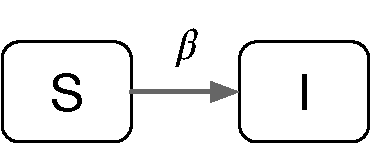
\includegraphics[width=0.3\textwidth]{pics/SI.pdf}
\end{textbox}





\begin{textbox}{SI - characteristics}
Each of the $i$ infected individuals infects in average $\beta$ contacts, but only $s=(1-i)$ of its contacts are indeed susceptible. More formally using differential equations:
% The expected number of contacts between Infected and Susceptible at any time is $is$, thus:

\begin{tabular}{p{0.07\textwidth}|p{0.8\textwidth}}\scriptsize

$\frac{di}{dt}$ & \textbf{Rate of new infection}: $\frac{di}{dt}=\beta i s=\beta (1-i)i$ \\


$i(t)$ & \textbf{Infected fraction}\footcite{barrat2008dynamical}: $i(t)=\frac{i_0e^{\beta t}}{1-i_0+i_0e^{\beta t}}$\\
$s(t)$ & \textbf{Susceptible fraction}: $1-i(t)$

\end{tabular}
The process can be separated in three steps:
\begin{itemize}
    \item At first, the fraction of infected individuals \textbf{Grows exponentially} until a large fraction of the population is infected. ($i$ is small,  $\frac{di}{dt}\approx \beta i \Rightarrow$ exponential)
    \item Due to \textbf{saturation}, the infection of the last individuals is slow
    \item The growth is faster and faster until half the population is infected ($\argmax_ {x,y}(x(1-x)):x=y=0.5$).
\end{itemize}


% In early times, the growth can seem slow

If $\beta>0$, everyone is infected at the end of the process.

\end{textbox}

\begin{textbox}{SI - Sketch}

\centering
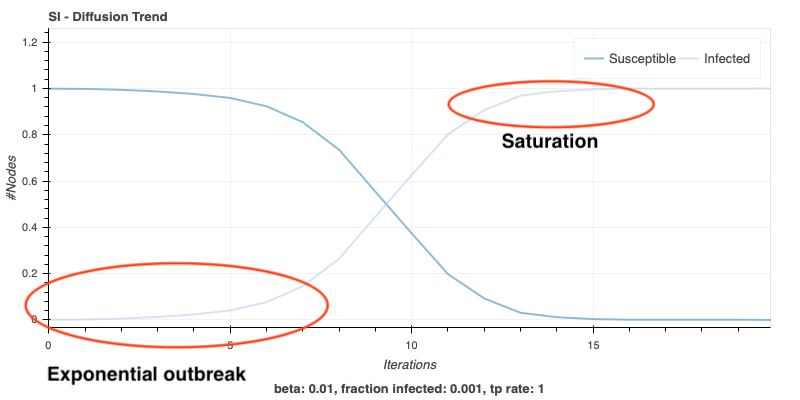
\includegraphics[width=0.9\textwidth]{pics/SIXP.png}
\end{textbox}

\begin{textbox}{SI - Application}
An example in which this model can be appropriate is for diffusion of innovation: being infected means buying or using a new service, product or technology whose usage becomes widespread in society, e.g., television, cell-phone, internet, Netflix, etc.

\centering

%\includegraphics[width=0.7\textwidth]{pics/SIadoption.png}
\colorbox{white}{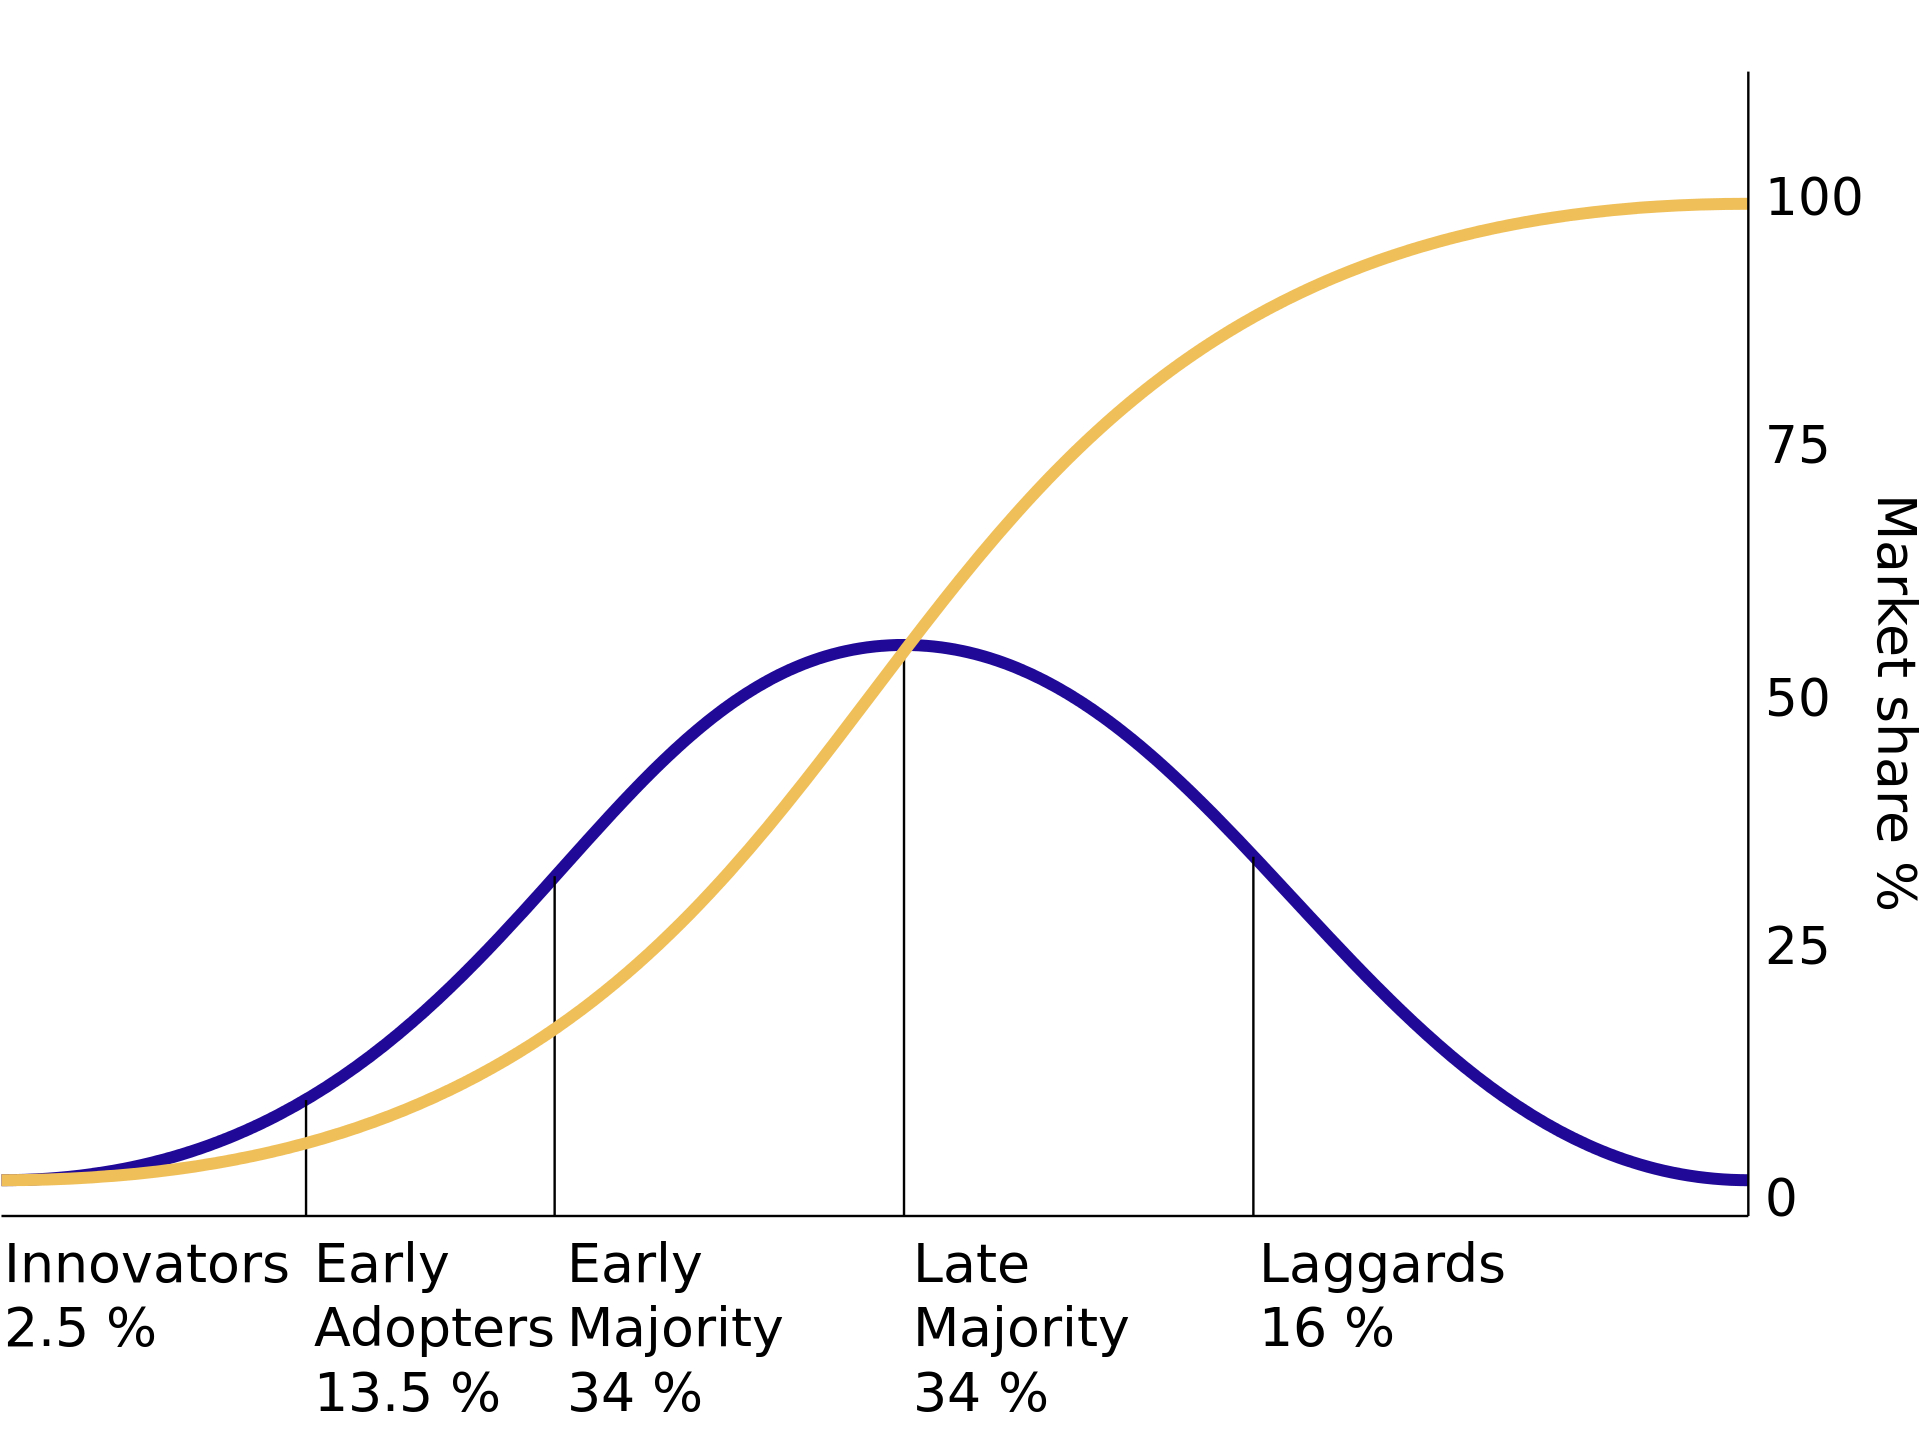
\includegraphics[width=0.7\textwidth]{pics/Diffusion_of_ideas.png}}

Illustration of Rogers's innovation adoption model. Image source\footnote{\url{https://en.wikipedia.org/wiki/Diffusion_of_innovations}}
\end{textbox}











\begin{textbox}{SIS}

When modeling real viruses, it is often useful to consider that infected individuals can \textbf{recover}, i.e., go back to the susceptible state, without becoming immune, such as for common cold or influenza. This can be modeled using the \textbf{SIS} model.

Additionally to $\beta$, the SIS model requires another parameter:

\begin{tabular}{p{0.07\textwidth}|p{0.8\textwidth}}\scriptsize

$\mu$ & \textbf{recovery rate}: probability that an \textit{Infected} individual go back to the susceptible state per unit of time.
\end{tabular}
\centering
\vspace{0.3cm}
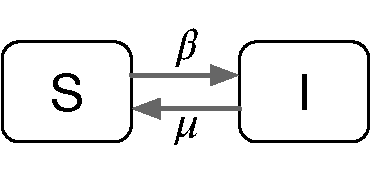
\includegraphics[width=0.3\textwidth]{pics/SIS.pdf}
\end{textbox}


\begin{textbox}{SIS - characteristics}
Intuitively, the fraction of infected individuals is now reduced by those switching to the susceptible state, more formally:
% The expected number of contacts between Infected and Susceptible at any time is $is$, thus:

% \begin{tabular}{p{0.07\textwidth}|p{0.8\textwidth}}\scriptsize
\begin{tabular}{p{0.07\textwidth}|p{0.8\textwidth}}\scriptsize

$\frac{di}{dt}$ & \textbf{Rate of new infection}: $\beta i(1-i) - \mu i=i(\beta - \mu - \beta i)$ \\



$i(t)$ & \textbf{Infected fraction\footcite{barrat2008dynamical}}: $\left( 1-\frac{\mu}{\beta }\right) \frac{Ce^{(\beta-\mu)t}}{1+Ce^{\beta-\mu)t}}$ \\

\end{tabular}


For large times, $i(t)\to 1-\frac{\mu}{\beta}$, i.e., the fraction of infected individuals stabilize around a value which depends only of parameters $\mu$ and $\beta$. 



% $i(t)$ & \textbf{Infected fraction}: $i(t)=\frac{i_0e^{\beta t}}{1-i_0+i_0e^{\beta t}}$

% \end{tabular}
\end{textbox}



\begin{textbox}{SIS - Sketch}

\centering
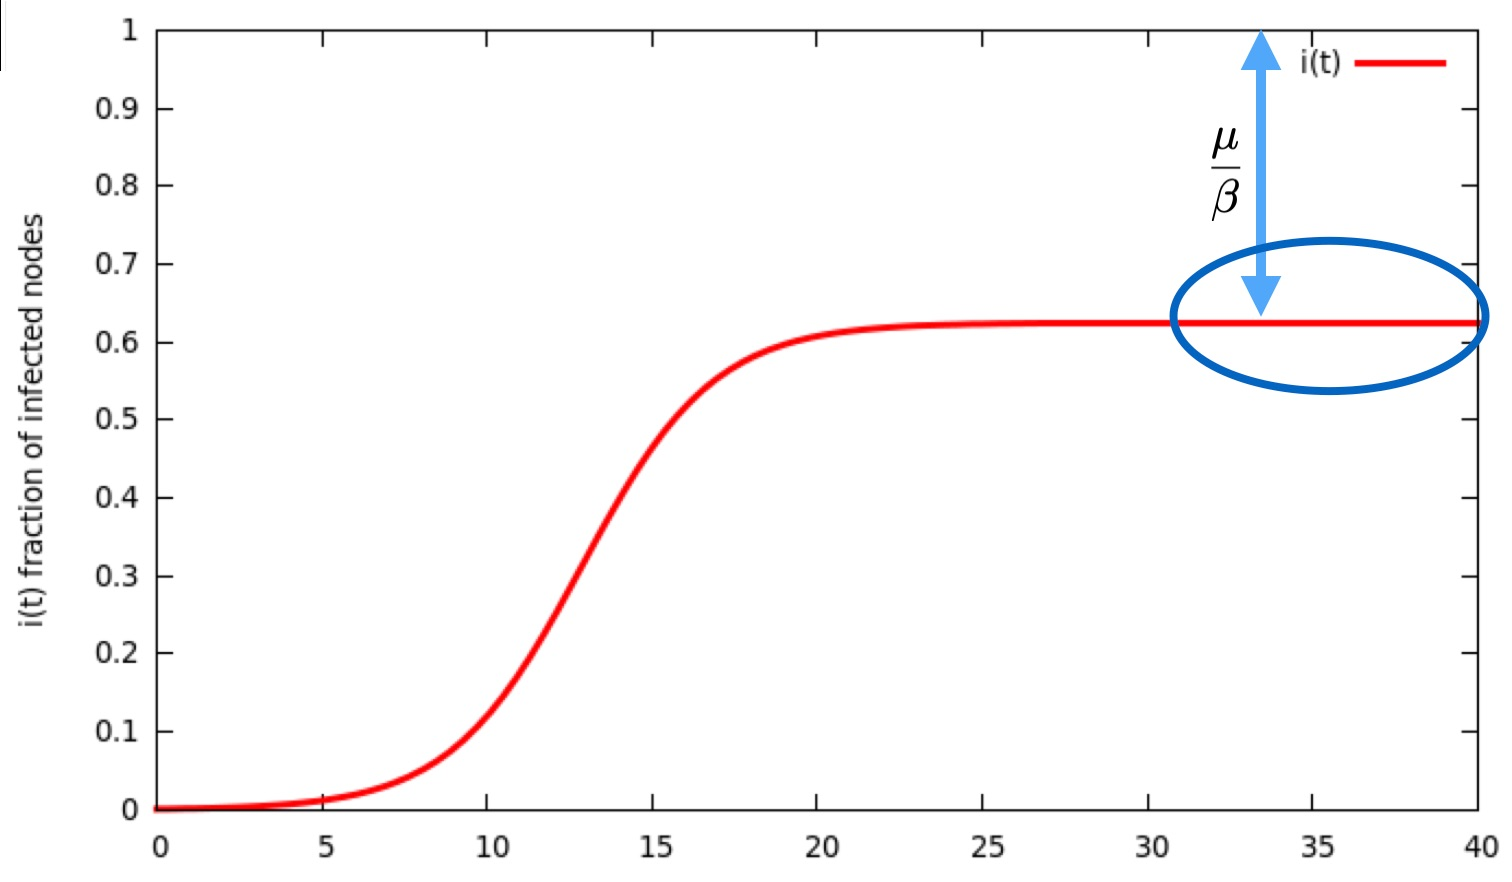
\includegraphics[width=0.9\textwidth]{pics/sisschema.jpg}
\end{textbox}












\begin{textbox}{$\lambda$ ratio or $(R_0)$}
In the SIS model, an important notion is the $\lambda$ ratio, also called $R_0$. 
\[
R_0=\frac{\beta}{\mu}
\]

$R_0$ can be understood as the average number of individuals that will be infected by an infected individual, \textbf{in a population in which all other nodes are Susceptible}. $R_0$ is a property of the model and \textbf{do not change with time}.

Looking at the $R_0$ is important in the early stage of the epidemic: 
\begin{itemize}
    \item if $R_0>1$, \textbf{there will be an outbreak}
    \item if $R_0<1$, \textbf{the epidemic will disappear naturally}.
\end{itemize}

If $R_0$ is just above 1, the outbreak also can stop naturally by chance in the early stage.
\end{textbox}
















\begin{textbox}{SIR}

In many spreading situations, infected individuals can themselves switch to a new state, usually called \textbf{Recovered}, which can represent either an acquired immunization or its removal (death, computer failure, etc.). In any case, Recovered individuals cannot infect nor be infected.

Additionally to $\beta$, the SIR model requires another parameter:

\begin{tabular}{p{0.07\textwidth}|p{0.8\textwidth}}\scriptsize

$\gamma$ & \textbf{recovery rate}: probability that an \textit{Infected} individual switch to the Recovered state per unit of time.
\end{tabular}
\centering
\vspace{0.3cm}
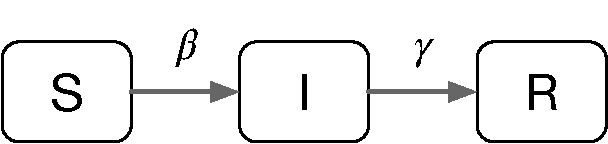
\includegraphics[width=0.6\textwidth]{pics/SIR.pdf}
\end{textbox}











\begin{textbox}{SIR - characteristics}
Intuitively, the fraction of infected individuals is now reduced by those switching to the recoved state, more formally:
% The expected number of contacts between Infected and Susceptible at any time is $is$, thus:

% \begin{tabular}{p{0.07\textwidth}|p{0.8\textwidth}}\scriptsize
\[
\frac{ds}{dt}=-\beta i s ,
\frac{di}{dt}=\beta i s- \gamma i,
\frac{dr}{dt}= \gamma i
\]

\begin{itemize}
    \item The initial steps of the outbreak still follow an exponential growth
    \item The fraction of infected nodes reach a peak and then decreases
    \item The fraction of recovered can saturate below 1
    \item The $\lambda$ ratio is defined as $\lambda=\frac{\beta}{\gamma}$
\end{itemize}

% $i(t)$ & \textbf{Infected fraction}: $i(t)=\frac{i_0e^{\beta t}}{1-i_0+i_0e^{\beta t}}$

% \end{tabular}
\end{textbox}



\begin{textbox}{SIR - sketch}


\centering
\colorbox{white}{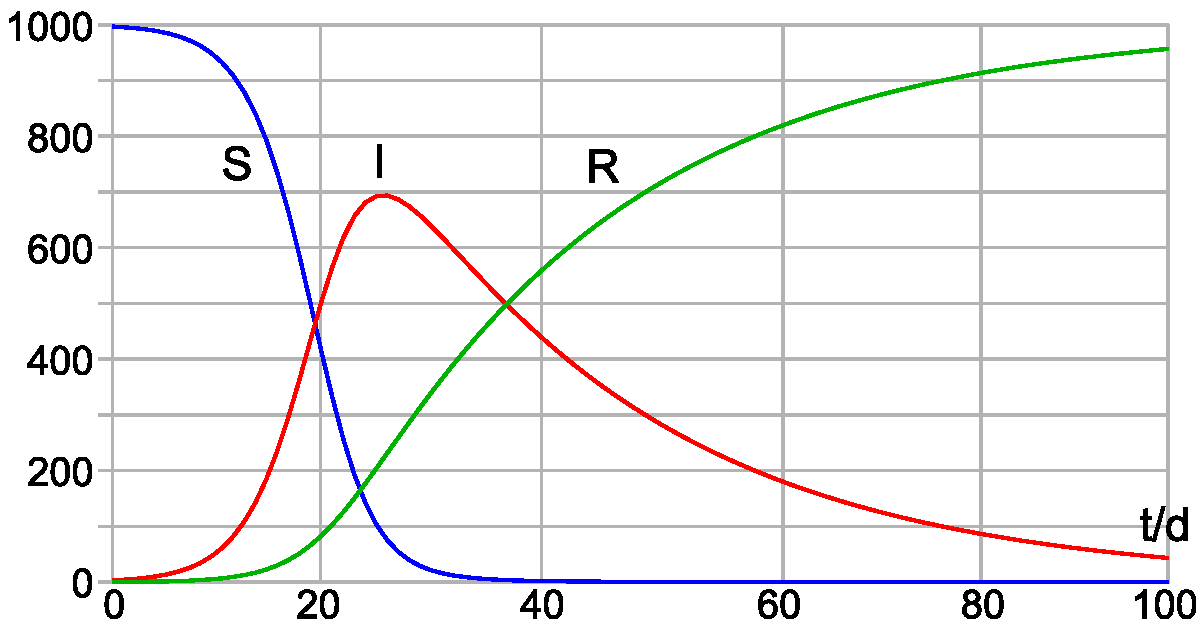
\includegraphics[width=0.7\textwidth]{pics/SIR-Modell.pdf}}

Image source: \footnote{\url{https://en.wikipedia.org/wiki/Compartmental_models_in_epidemiology}}


\end{textbox}
% \begin{textbox}{SIR - $\lambda$ or $(R_0)$}
% In the SIR model, 
% \[
% R_0=\frac{\beta}{\gamma}
% \]

% $R_0$ can be understood as the average number of individuals that will be infected by an infected individual, \textbf{in a population in which all other nodes are Susceptible}. $R_0$ is a property of the model and do not change with time.

% Looking at the $R_0$ is important in the early stage of the epidemic: 
% \begin{itemize}
%     \item if $R_0>1$, \textbf{there will be an outbreak}
%     \item if $R_0<1$, \textbf{the epidemic will disappear naturally}.
% \end{itemize}

% If $R_0$ is just above 1, the outbreak also can stop naturally by chance in the early stage.
% \end{textbox}





\begin{textbox}{Other non-network models}
Epidemic modeling is a large and rich scientific topic, thus those models are nowadays considered \textit{toy models}, too simple to model real epidemics. Most used model thus include other factors, such as \textbf{natural population dynamic} (birth, natural death, etc. for long term dynamics), \textbf{population segmentation} ($tau$ might differ among subsets of populations, e.g., elderly, maried couples, etc.), \textbf{population mixing} ($\hat{c}$ might vary between members of a subpopulation and another), etc.
\end{textbox}

\begin{textbox}{Network models}
A natural way to add more details to a spreading process is, instead of considering an homogeneous population, or a population composed of homogeneous subpopulations, to study the diffusion on a network representing the structure of the population.


\end{textbox}



\begin{textbox}{Notation change on networks}
$\hat{c}$ has no meaning in networks (its role is played by the network structure), so by convention we use $\beta=\tau$ : the probability for a node to infect each of its neighbor at each step.

\end{textbox}

\begin{textbox}{Homogeneous Networks}
If we consider an \textbf{homogeneous random network} in which all nodes have degree exactly $k$, then we can consider the spreading on this network as similar to the non-network models, with $\hat{c}=k$. 

For instance, the SI model becomes:
\[
\frac{di}{dt}=\beta \langle k \rangle (1-i)i
\]

Note that in practice, there are a few differences, such as a switch from a continuous to a discrete setting, but they have no consequences on large graphs.

\end{textbox}




\begin{textbox}{ER Networks}
In ER random graphs, for large graphs, we have seen that $k\approx \langle k \rangle$, thus the same model description still holds, with the approximation being better for larger networks.

\end{textbox}

\begin{textbox}{$R_0$ on networks}
In homogeneous or ER networks, $R_0$ is naturally defined as $\frac{\beta \langle k \rangle}{\mu}$
    
Another way to express the same thing is that, if we define $R_0=\frac{\beta}{\mu}$, then the epidemic threshold is not equal to 1 but to $\frac{1}{\langle k \rangle}$
    
\end{textbox}











\begin{textbox}{Heterogeneous Degrees - Degree blocks}
We have seen that most real networks have an heterogeneous degree distribution. To study analytically the effect of this property, a method is to use a \textbf{degree block approximation}: we consider all nodes with a given degree as an homogeneous groups(degree block), and analyze each of these groups separately.

$i_k,s_k,r_k$: fractions of nodes of degree $k$ that are infected, susceptible, recovered, respectively.

The global average is the average for all degree block, weighted by the fraction of nodes in each block.
$i=\sum_k P(k)i_k$
with $P(k)$ the fraction of nodes having degree $k$.

The same holds for global $s$ and $r$.
\end{textbox}




\begin{textbox}{Heterogeneous Degrees - SI}


For the SI model, we know that all nodes are infected in the end, but what may vary is \textbf{speed} of the process.

The speed of diffusion by degree block can be expressed as:
\[
\frac{di_k}{dt}= \beta k(1-i_k) \Theta_k
\]
with $\Theta_k$ being the fraction of infected neighbors of a node with degree $k$.

\end{textbox}


\begin{textbox}{Heterogeneous Degrees - $\Theta_k$}
$\Theta_k$ represents the fraction of infected neighbors of a node with degree $k$. If the network is homogeneous, $\Theta_k(t)=i(t)$. If the graph is heterogeneous, nodes with different degrees have different probabilities of being infected: higher degree nodes are, by definition, more exposed, since they have more chances of being infected at each step. 

This is important for two reasons:
\begin{itemize}
    \item Due to the friendship paradox, nodes are more likely to be connected to large nodes than to small ones
    \item In real networks, we have seen that there is often a degree assortativity, thus nodes of a given degree have different degrees in their neighborhood.
\end{itemize}

We can thus define $\Theta_k$ as the probability to be connected to nodes of a given degree and or their respective probability of being infected $\Theta_k=\sum_{k'}P(k'|k)i_{k'}$, with $P(k'|k)$ the probability that a node with degree $k$ connects to a node with degree $k'$.

For simplicity, \textbf{we assume no degree-degree correlation}.

$P(k'|k)$ can then be expressed as the fraction of all edge stubs attached to nodes of degree $k'$, indepedent of the $k$ under study:

%\Theta_k=\sum_{k'}P(k'|k)i_k'
\[
P(k'|k)=\frac{k'P(k')}{\sum_{k''}k''P(k'')}=\frac{k'P(k')}{\langle k \rangle}
\]

% And the fraction of infected neighbors do not depend on the degree of the node, but only on the probability to be connected to nodes of a given degree and or their respective probability of being infected.
And: 
\[
\Theta_k=\Theta= \frac{\sum_{k'}k' P(k')i_{k'}}{\langle k \rangle}
\]
% Note the $(k'-1)$ in the equation: we compute the fraction of infected nodes in the neighborhood of susceptible nodes. Among the neighbors of each 


\end{textbox}




\begin{textbox}{Heterogeneous Degrees - SI - time scale}

From previous equations, it can be shown\footcite{barrat2008dynamical} that the \textbf{time scale} $\tau$ of the process, i.e., a measure inversely proportional to its speed, is $\tau=\frac{\langle k \rangle}{\beta(\langle k^2 \rangle - \langle k \rangle)}$. 

Thus, for a given average degree $\langle k \rangle$ and a given $\beta$, \textbf{the more heterogeneous the degrees, the faster the diffusion}.

If the degree distribution follows a power law of exponent $\alpha<3$, we have seen that $\langle k^2 \rangle$ diverge towards infinity, thus $\tau$ tends toward 0, thus the diffusion is nearly instantaneous.

This can be understood as follows: if a node is connected to nearly every other node, then it has an extremely high probability to become infected immediately, and can then infect the rest of the network extremely quickly.

\end{textbox}



\begin{textbox}{Heterogeneous Degrees - $\lambda$}

For SIS and SIR models, it can also be shown \footcite{barrat2008dynamical} that the epidemic threshold $\lambda$ (or $R_0$) is not reached when $\lambda=\frac{\beta\langle k \rangle}{\mu}>1$ as in homogeneous networks, but when $\lambda >\frac{\langle k \rangle^2}{\langle k^2 \rangle}$.

This means that in a very heterogeneous network, \textbf{an outbreak can start even if $\lambda$ is very small, and below 1}. 

Intuitively, even if people recover faster than they spread the virus in average, some nodes (hubs) will nevertheless become infected, and since they can infect many others, the contagion will spread.

%Fortunately, it can also be shown that such an outbreak will stop way before reaching all nodes%\footcite{barrat2008dynamical}.

\end{textbox}



% \begin{textbox}{WS Networks}
% In WS random graphs, it has been observed empirically \footcite{watts1998collective} that raising the fraction of \textit{shortcuts} (the random rewiring probability) quickly raises the speed of the diffusion. It is difficult to describe analytically this phenomenon due to the mixed effect of an increased variance in degree distribution, a decrease in the clustering coefficient and a decrease in the average distance.




















% \end{textbox}
\begin{textbox}{SIR - Experimental}
When analytical solutions cannot be simply derived, empirical simulations can be used to observe the effect of network properties on diffusion processes. 

In particular, these properties can be used to asses the effect of typical heterogeneity: degree-heterogeneity, belonging to blocks, spatial heterogeneity, etc.
\end{textbox}

\begin{textbox}{SIR - Community Structure}
In this experiment, we compare an ER network to Stochastic Block Models. 

\textbf{Network parameters}: $n=1000,\langle k \rangle=5$.

\textbf{SBM parameters} Number of blocks $|C|= 100$.  We vary $L^{in}$, the fraction of all edges that are inside blocks. When $L^{in}=0.01,p^{in} \approx p^{out}=0.005$. When $L^{in}=0.9, p^{in}=0.5,p^{out}\approx0.0005$


\textbf{SIR parameters}: $\theta=0.2$,$\gamma=0.5$.
The initial number of infected nodes is 5, all of them in the same community structure.

\centering
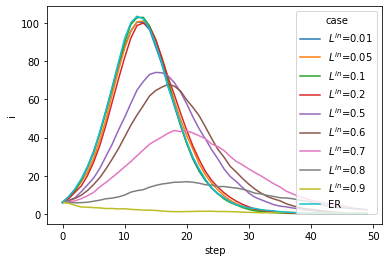
\includegraphics[width=0.7\textwidth]{pics/sir_com.png}

We observe that the more marked the communities, the less efficient the spreading process.

\end{textbox}


\begin{textbox}{SIR - Scale Free}
In this experiment, we compare an ER network to Configuration Models with power law degree distributions. 

\textbf{Network parameters}:$n=1000,\langle k \rangle=5$. We vary the exponent of the distribution, while keeping $\langle k \rangle=5$ constant.

\textbf{SIR parameters}: $\theta=0.2$,$\gamma=0.5$.
The initial number of infected nodes is 5, all of them in the same community structure.

\centering
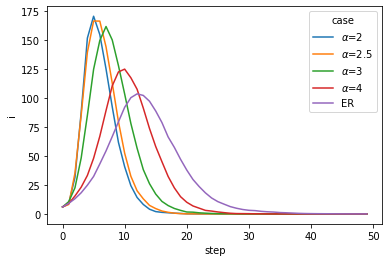
\includegraphics[width=0.7\textwidth]{pics/SIRpowerlaw.png}

The highest the exponent of the degree distribution, the faster is the diffusion.

\end{textbox}

\begin{textbox}{SIR - Spatial effect - WS}
In this experiment, we compare an ER network to Watts Strogatz random graphs, varying the probability of rewiring edges. It can be understood as a model of spatial proximity: with $p=0$, each node is connected only to its direct neighbors in the 1 dimensional space. If $p=1$, each node is connected to exactly $k$ random nodes.

\textbf{Network parameters}:$n=1000,\langle k \rangle=5$

\textbf{SIR parameters}: $\theta=0.2$,$\gamma=0.5$.
The initial number of infected nodes is 5, being 5 direct neighbors.

\centering

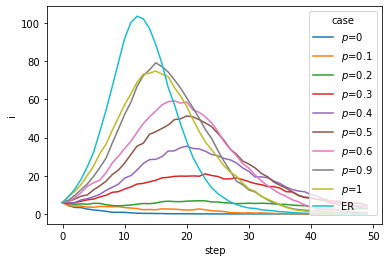
\includegraphics[width=0.7\textwidth]{pics/SIR_WS.png}

The more nodes tend to be connected to direct neighbors in space, the slower the diffusion. 
%Note that the difference with an ER model in those simulations comes from the constant degree of nodes.

\end{textbox}

\begin{textbox}{Application of diffusion models}
Diffusion models can be used for several applications: 
\begin{itemize}
    \item Model fitting: better understand an actual epidemic by fitting parameters on real observations
    \item Predicting trends of evolution 
    \item Control of epidemics: Given an epidemic model and a supporting network, find an optimal solution to control (accelerate or slow-down) the epidemic.
\end{itemize}

\end{textbox}


\begin{textbox}{Optimal node/edge removal}
One way to slow-down an epidemic consist in \textbf{removing nodes}(e.g., vaccination). The problem can be formulated as a budget constrained removal, i.e., if we can remove only $x$ nodes/edges, which one should we choose? Based on theoretical and experimental results, heuristic solutions consist in removing: \textbf{highest degree nodes}, \textbf{highest betweeness} nodes/edges (isolating communities), long-distance edges (shortcuts) in spatial networks. 
\end{textbox}

\begin{textbox}{Friendship paradox and node removal}
It has been proposed\footcite{cohen2003efficient} that the friendship paradox could be used to apply budget-constrained high degree nodes preferential vaccination in real networks where finding such nodes is not possible because the whole network is unknown: instead of targeting random individuals, one could vaccinate random contacts of random individuals, thus greatly increasing the average degree of vaccinated persons.
\end{textbox}

% \begin{textbox}{Control of epidemics}
% Controlling an epidemic can be done using\footcite{nowzari2016analysis}:
% \begin{itemize}
%     \item Optimal Node Removal
%     \item Optimal Link Removal
%     \item Budget Constrained 
% \end{itemize}

% \end{textbox}



\begin{textbox}{Going further}
Book Dynamic processes on Networks: \cite{barrat2008dynamical}

Surveys:

Analysis and Control of Epidemics: \cite{nowzari2016analysis}

Diffusion in networks: \cite{lamberson2016diffusion}

Impact of community structure: \cite{stegehuis2016epidemic}
\end{textbox}

 \AtNextBibliography{\footnotesize}


\printbibliography[heading=subbibliography]


\end{multicols}



\end{document}


